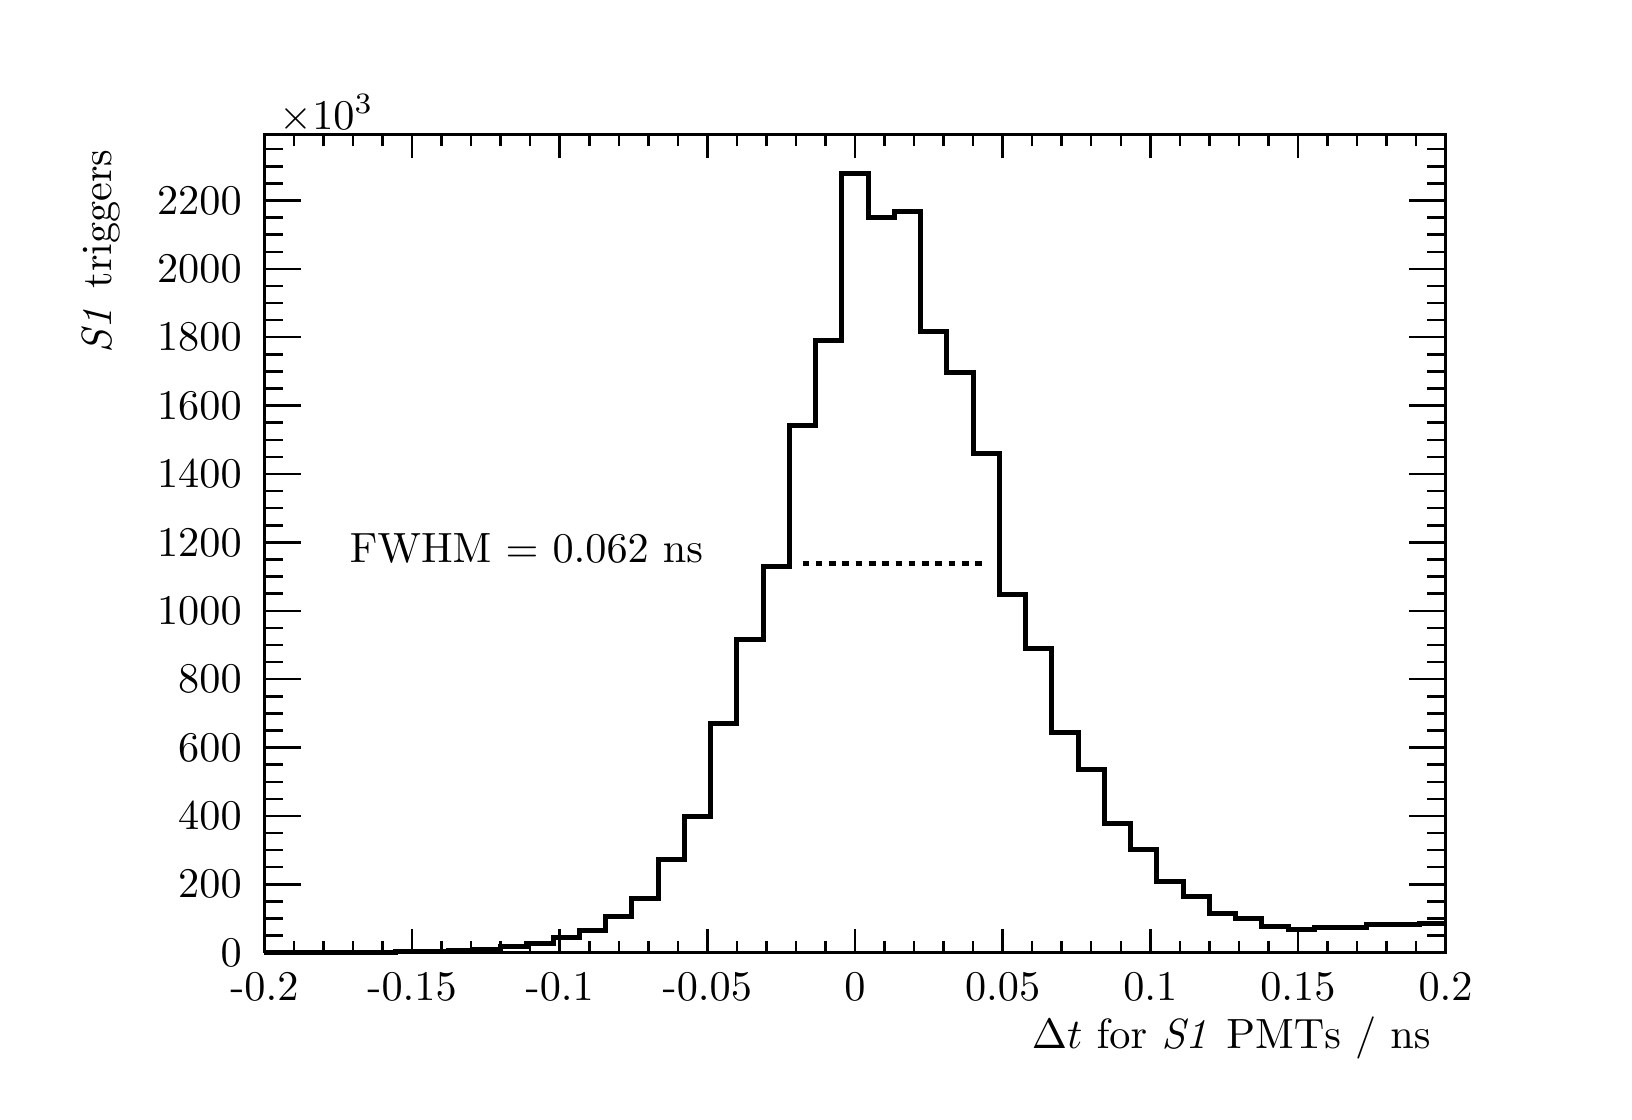
\begin{tikzpicture}
\pgfdeclareplotmark{cross} {
\pgfpathmoveto{\pgfpoint{-0.3\pgfplotmarksize}{\pgfplotmarksize}}
\pgfpathlineto{\pgfpoint{+0.3\pgfplotmarksize}{\pgfplotmarksize}}
\pgfpathlineto{\pgfpoint{+0.3\pgfplotmarksize}{0.3\pgfplotmarksize}}
\pgfpathlineto{\pgfpoint{+1\pgfplotmarksize}{0.3\pgfplotmarksize}}
\pgfpathlineto{\pgfpoint{+1\pgfplotmarksize}{-0.3\pgfplotmarksize}}
\pgfpathlineto{\pgfpoint{+0.3\pgfplotmarksize}{-0.3\pgfplotmarksize}}
\pgfpathlineto{\pgfpoint{+0.3\pgfplotmarksize}{-1.\pgfplotmarksize}}
\pgfpathlineto{\pgfpoint{-0.3\pgfplotmarksize}{-1.\pgfplotmarksize}}
\pgfpathlineto{\pgfpoint{-0.3\pgfplotmarksize}{-0.3\pgfplotmarksize}}
\pgfpathlineto{\pgfpoint{-1.\pgfplotmarksize}{-0.3\pgfplotmarksize}}
\pgfpathlineto{\pgfpoint{-1.\pgfplotmarksize}{0.3\pgfplotmarksize}}
\pgfpathlineto{\pgfpoint{-0.3\pgfplotmarksize}{0.3\pgfplotmarksize}}
\pgfpathclose
\pgfusepathqstroke
}
\pgfdeclareplotmark{cross*} {
\pgfpathmoveto{\pgfpoint{-0.3\pgfplotmarksize}{\pgfplotmarksize}}
\pgfpathlineto{\pgfpoint{+0.3\pgfplotmarksize}{\pgfplotmarksize}}
\pgfpathlineto{\pgfpoint{+0.3\pgfplotmarksize}{0.3\pgfplotmarksize}}
\pgfpathlineto{\pgfpoint{+1\pgfplotmarksize}{0.3\pgfplotmarksize}}
\pgfpathlineto{\pgfpoint{+1\pgfplotmarksize}{-0.3\pgfplotmarksize}}
\pgfpathlineto{\pgfpoint{+0.3\pgfplotmarksize}{-0.3\pgfplotmarksize}}
\pgfpathlineto{\pgfpoint{+0.3\pgfplotmarksize}{-1.\pgfplotmarksize}}
\pgfpathlineto{\pgfpoint{-0.3\pgfplotmarksize}{-1.\pgfplotmarksize}}
\pgfpathlineto{\pgfpoint{-0.3\pgfplotmarksize}{-0.3\pgfplotmarksize}}
\pgfpathlineto{\pgfpoint{-1.\pgfplotmarksize}{-0.3\pgfplotmarksize}}
\pgfpathlineto{\pgfpoint{-1.\pgfplotmarksize}{0.3\pgfplotmarksize}}
\pgfpathlineto{\pgfpoint{-0.3\pgfplotmarksize}{0.3\pgfplotmarksize}}
\pgfpathclose
\pgfusepathqfillstroke
}
\pgfdeclareplotmark{newstar} {
\pgfpathmoveto{\pgfqpoint{0pt}{\pgfplotmarksize}}
\pgfpathlineto{\pgfqpointpolar{44}{0.5\pgfplotmarksize}}
\pgfpathlineto{\pgfqpointpolar{18}{\pgfplotmarksize}}
\pgfpathlineto{\pgfqpointpolar{-20}{0.5\pgfplotmarksize}}
\pgfpathlineto{\pgfqpointpolar{-54}{\pgfplotmarksize}}
\pgfpathlineto{\pgfqpointpolar{-90}{0.5\pgfplotmarksize}}
\pgfpathlineto{\pgfqpointpolar{234}{\pgfplotmarksize}}
\pgfpathlineto{\pgfqpointpolar{198}{0.5\pgfplotmarksize}}
\pgfpathlineto{\pgfqpointpolar{162}{\pgfplotmarksize}}
\pgfpathlineto{\pgfqpointpolar{134}{0.5\pgfplotmarksize}}
\pgfpathclose
\pgfusepathqstroke
}
\pgfdeclareplotmark{newstar*} {
\pgfpathmoveto{\pgfqpoint{0pt}{\pgfplotmarksize}}
\pgfpathlineto{\pgfqpointpolar{44}{0.5\pgfplotmarksize}}
\pgfpathlineto{\pgfqpointpolar{18}{\pgfplotmarksize}}
\pgfpathlineto{\pgfqpointpolar{-20}{0.5\pgfplotmarksize}}
\pgfpathlineto{\pgfqpointpolar{-54}{\pgfplotmarksize}}
\pgfpathlineto{\pgfqpointpolar{-90}{0.5\pgfplotmarksize}}
\pgfpathlineto{\pgfqpointpolar{234}{\pgfplotmarksize}}
\pgfpathlineto{\pgfqpointpolar{198}{0.5\pgfplotmarksize}}
\pgfpathlineto{\pgfqpointpolar{162}{\pgfplotmarksize}}
\pgfpathlineto{\pgfqpointpolar{134}{0.5\pgfplotmarksize}}
\pgfpathclose
\pgfusepathqfillstroke
}
\definecolor{c}{rgb}{1,1,1};
\draw [color=c, fill=c] (0,0) rectangle (20,13.4957);
\draw [color=c, fill=c] (3,1.75444) rectangle (18,12.1461);
\definecolor{c}{rgb}{0,0,0};
\draw [c,line width=0.9] (3,1.75444) -- (3,12.1461) -- (18,12.1461) -- (18,1.75444) -- (3,1.75444);
\definecolor{c}{rgb}{1,1,1};
\draw [color=c, fill=c] (3,1.75444) rectangle (18,12.1461);
\definecolor{c}{rgb}{0,0,0};
\draw [c,line width=0.9] (3,1.75444) -- (3,12.1461) -- (18,12.1461) -- (18,1.75444) -- (3,1.75444);
\draw [c,line width=1.8] (3,1.75651) -- (3.33333,1.75651) -- (3.33333,1.75672) -- (3.66667,1.75672) -- (3.66667,1.75782) -- (4,1.75782) -- (4,1.75928) -- (4.33333,1.75928) -- (4.33333,1.76265) -- (4.66667,1.76265) -- (4.66667,1.76637) -- (5,1.76637)
 -- (5,1.77413) -- (5.33333,1.77413) -- (5.33333,1.78786) -- (5.66667,1.78786) -- (5.66667,1.80025) -- (6,1.80025) -- (6,1.83002) -- (6.33333,1.83002) -- (6.33333,1.8656) -- (6.66667,1.8656) -- (6.66667,1.94289) -- (7,1.94289) -- (7,2.03217) --
 (7.33333,2.03217) -- (7.33333,2.21951) -- (7.66667,2.21951) -- (7.66667,2.44174) -- (8,2.44174) -- (8,2.9414) -- (8.33333,2.9414) -- (8.33333,3.48698) -- (8.66667,3.48698) -- (8.66667,4.66096) -- (9,4.66096) -- (9,5.73419) -- (9.33333,5.73419) --
 (9.33333,6.66117) -- (9.66667,6.66117) -- (9.66667,8.44555) -- (10,8.44555) -- (10,9.52377) -- (10.3333,9.52377) -- (10.3333,11.6513) -- (10.6667,11.6513) -- (10.6667,11.0943) -- (11,11.0943) -- (11,11.169) -- (11.3333,11.169) -- (11.3333,9.64689)
 -- (11.6667,9.64689) -- (11.6667,9.12428) -- (12,9.12428) -- (12,8.09889) -- (12.3333,8.09889) -- (12.3333,6.29961) -- (12.6667,6.29961) -- (12.6667,5.61671) -- (13,5.61671) -- (13,4.54715) -- (13.3333,4.54715) -- (13.3333,4.0756) --
 (13.6667,4.0756) -- (13.6667,3.39822) -- (14,3.39822) -- (14,3.07106) -- (14.3333,3.07106) -- (14.3333,2.65631) -- (14.6667,2.65631) -- (14.6667,2.46793) -- (15,2.46793) -- (15,2.25342) -- (15.3333,2.25342) -- (15.3333,2.18649) -- (15.6667,2.18649)
 -- (15.6667,2.08911) -- (16,2.08911) -- (16,2.05201) -- (16.3333,2.05201) -- (16.3333,2.07377) -- (16.6667,2.07377) -- (16.6667,2.07323) -- (17,2.07323) -- (17,2.1138) -- (17.3333,2.1138) -- (17.3333,2.11352) -- (17.6667,2.11352) --
 (17.6667,2.12843) -- (18,2.12843);
\draw [c,line width=0.9] (3,1.75444) -- (18,1.75444);
\draw [c,line width=0.9] (3,2.05809) -- (3,1.75444);
\draw [c,line width=0.9] (3.375,1.90627) -- (3.375,1.75444);
\draw [c,line width=0.9] (3.75,1.90627) -- (3.75,1.75444);
\draw [c,line width=0.9] (4.125,1.90627) -- (4.125,1.75444);
\draw [c,line width=0.9] (4.5,1.90627) -- (4.5,1.75444);
\draw [c,line width=0.9] (4.875,2.05809) -- (4.875,1.75444);
\draw [c,line width=0.9] (5.25,1.90627) -- (5.25,1.75444);
\draw [c,line width=0.9] (5.625,1.90627) -- (5.625,1.75444);
\draw [c,line width=0.9] (6,1.90627) -- (6,1.75444);
\draw [c,line width=0.9] (6.375,1.90627) -- (6.375,1.75444);
\draw [c,line width=0.9] (6.75,2.05809) -- (6.75,1.75444);
\draw [c,line width=0.9] (7.125,1.90627) -- (7.125,1.75444);
\draw [c,line width=0.9] (7.5,1.90627) -- (7.5,1.75444);
\draw [c,line width=0.9] (7.875,1.90627) -- (7.875,1.75444);
\draw [c,line width=0.9] (8.25,1.90627) -- (8.25,1.75444);
\draw [c,line width=0.9] (8.625,2.05809) -- (8.625,1.75444);
\draw [c,line width=0.9] (9,1.90627) -- (9,1.75444);
\draw [c,line width=0.9] (9.375,1.90627) -- (9.375,1.75444);
\draw [c,line width=0.9] (9.75,1.90627) -- (9.75,1.75444);
\draw [c,line width=0.9] (10.125,1.90627) -- (10.125,1.75444);
\draw [c,line width=0.9] (10.5,2.05809) -- (10.5,1.75444);
\draw [c,line width=0.9] (10.875,1.90627) -- (10.875,1.75444);
\draw [c,line width=0.9] (11.25,1.90627) -- (11.25,1.75444);
\draw [c,line width=0.9] (11.625,1.90627) -- (11.625,1.75444);
\draw [c,line width=0.9] (12,1.90627) -- (12,1.75444);
\draw [c,line width=0.9] (12.375,2.05809) -- (12.375,1.75444);
\draw [c,line width=0.9] (12.75,1.90627) -- (12.75,1.75444);
\draw [c,line width=0.9] (13.125,1.90627) -- (13.125,1.75444);
\draw [c,line width=0.9] (13.5,1.90627) -- (13.5,1.75444);
\draw [c,line width=0.9] (13.875,1.90627) -- (13.875,1.75444);
\draw [c,line width=0.9] (14.25,2.05809) -- (14.25,1.75444);
\draw [c,line width=0.9] (14.625,1.90627) -- (14.625,1.75444);
\draw [c,line width=0.9] (15,1.90627) -- (15,1.75444);
\draw [c,line width=0.9] (15.375,1.90627) -- (15.375,1.75444);
\draw [c,line width=0.9] (15.75,1.90627) -- (15.75,1.75444);
\draw [c,line width=0.9] (16.125,2.05809) -- (16.125,1.75444);
\draw [c,line width=0.9] (16.5,1.90627) -- (16.5,1.75444);
\draw [c,line width=0.9] (16.875,1.90627) -- (16.875,1.75444);
\draw [c,line width=0.9] (17.25,1.90627) -- (17.25,1.75444);
\draw [c,line width=0.9] (17.625,1.90627) -- (17.625,1.75444);
\draw [c,line width=0.9] (18,2.05809) -- (18,1.75444);
\draw [anchor=base] (3,1.14713) node[scale=1.52731, color=c, rotate=0]{-0.2};
\draw [anchor=base] (4.875,1.14713) node[scale=1.52731, color=c, rotate=0]{-0.15};
\draw [anchor=base] (6.75,1.14713) node[scale=1.52731, color=c, rotate=0]{-0.1};
\draw [anchor=base] (8.625,1.14713) node[scale=1.52731, color=c, rotate=0]{-0.05};
\draw [anchor=base] (10.5,1.14713) node[scale=1.52731, color=c, rotate=0]{0};
\draw [anchor=base] (12.375,1.14713) node[scale=1.52731, color=c, rotate=0]{0.05};
\draw [anchor=base] (14.25,1.14713) node[scale=1.52731, color=c, rotate=0]{0.1};
\draw [anchor=base] (16.125,1.14713) node[scale=1.52731, color=c, rotate=0]{0.15};
\draw [anchor=base] (18,1.14713) node[scale=1.52731, color=c, rotate=0]{0.2};
\draw [anchor= east] (18,0.674785) node[scale=1.52731, color=c, rotate=0]{$\Delta t$ for $\mathit{S1}$ PMTs / ns};
\draw [c,line width=0.9] (3,12.1461) -- (18,12.1461);
\draw [c,line width=0.9] (3,11.8425) -- (3,12.1461);
\draw [c,line width=0.9] (3.375,11.9943) -- (3.375,12.1461);
\draw [c,line width=0.9] (3.75,11.9943) -- (3.75,12.1461);
\draw [c,line width=0.9] (4.125,11.9943) -- (4.125,12.1461);
\draw [c,line width=0.9] (4.5,11.9943) -- (4.5,12.1461);
\draw [c,line width=0.9] (4.875,11.8425) -- (4.875,12.1461);
\draw [c,line width=0.9] (5.25,11.9943) -- (5.25,12.1461);
\draw [c,line width=0.9] (5.625,11.9943) -- (5.625,12.1461);
\draw [c,line width=0.9] (6,11.9943) -- (6,12.1461);
\draw [c,line width=0.9] (6.375,11.9943) -- (6.375,12.1461);
\draw [c,line width=0.9] (6.75,11.8425) -- (6.75,12.1461);
\draw [c,line width=0.9] (7.125,11.9943) -- (7.125,12.1461);
\draw [c,line width=0.9] (7.5,11.9943) -- (7.5,12.1461);
\draw [c,line width=0.9] (7.875,11.9943) -- (7.875,12.1461);
\draw [c,line width=0.9] (8.25,11.9943) -- (8.25,12.1461);
\draw [c,line width=0.9] (8.625,11.8425) -- (8.625,12.1461);
\draw [c,line width=0.9] (9,11.9943) -- (9,12.1461);
\draw [c,line width=0.9] (9.375,11.9943) -- (9.375,12.1461);
\draw [c,line width=0.9] (9.75,11.9943) -- (9.75,12.1461);
\draw [c,line width=0.9] (10.125,11.9943) -- (10.125,12.1461);
\draw [c,line width=0.9] (10.5,11.8425) -- (10.5,12.1461);
\draw [c,line width=0.9] (10.875,11.9943) -- (10.875,12.1461);
\draw [c,line width=0.9] (11.25,11.9943) -- (11.25,12.1461);
\draw [c,line width=0.9] (11.625,11.9943) -- (11.625,12.1461);
\draw [c,line width=0.9] (12,11.9943) -- (12,12.1461);
\draw [c,line width=0.9] (12.375,11.8425) -- (12.375,12.1461);
\draw [c,line width=0.9] (12.75,11.9943) -- (12.75,12.1461);
\draw [c,line width=0.9] (13.125,11.9943) -- (13.125,12.1461);
\draw [c,line width=0.9] (13.5,11.9943) -- (13.5,12.1461);
\draw [c,line width=0.9] (13.875,11.9943) -- (13.875,12.1461);
\draw [c,line width=0.9] (14.25,11.8425) -- (14.25,12.1461);
\draw [c,line width=0.9] (14.625,11.9943) -- (14.625,12.1461);
\draw [c,line width=0.9] (15,11.9943) -- (15,12.1461);
\draw [c,line width=0.9] (15.375,11.9943) -- (15.375,12.1461);
\draw [c,line width=0.9] (15.75,11.9943) -- (15.75,12.1461);
\draw [c,line width=0.9] (16.125,11.8425) -- (16.125,12.1461);
\draw [c,line width=0.9] (16.5,11.9943) -- (16.5,12.1461);
\draw [c,line width=0.9] (16.875,11.9943) -- (16.875,12.1461);
\draw [c,line width=0.9] (17.25,11.9943) -- (17.25,12.1461);
\draw [c,line width=0.9] (17.625,11.9943) -- (17.625,12.1461);
\draw [c,line width=0.9] (18,11.8425) -- (18,12.1461);
\draw [c,line width=0.9] (3,1.75444) -- (3,12.1461);
\draw [c,line width=0.9] (3.462,1.75444) -- (3,1.75444);
\draw [c,line width=0.9] (3.231,1.97157) -- (3,1.97157);
\draw [c,line width=0.9] (3.231,2.1887) -- (3,2.1887);
\draw [c,line width=0.9] (3.231,2.40582) -- (3,2.40582);
\draw [c,line width=0.9] (3.462,2.62295) -- (3,2.62295);
\draw [c,line width=0.9] (3.231,2.84008) -- (3,2.84008);
\draw [c,line width=0.9] (3.231,3.0572) -- (3,3.0572);
\draw [c,line width=0.9] (3.231,3.27433) -- (3,3.27433);
\draw [c,line width=0.9] (3.462,3.49146) -- (3,3.49146);
\draw [c,line width=0.9] (3.231,3.70859) -- (3,3.70859);
\draw [c,line width=0.9] (3.231,3.92571) -- (3,3.92571);
\draw [c,line width=0.9] (3.231,4.14284) -- (3,4.14284);
\draw [c,line width=0.9] (3.462,4.35997) -- (3,4.35997);
\draw [c,line width=0.9] (3.231,4.57709) -- (3,4.57709);
\draw [c,line width=0.9] (3.231,4.79422) -- (3,4.79422);
\draw [c,line width=0.9] (3.231,5.01135) -- (3,5.01135);
\draw [c,line width=0.9] (3.462,5.22847) -- (3,5.22847);
\draw [c,line width=0.9] (3.231,5.4456) -- (3,5.4456);
\draw [c,line width=0.9] (3.231,5.66273) -- (3,5.66273);
\draw [c,line width=0.9] (3.231,5.87986) -- (3,5.87986);
\draw [c,line width=0.9] (3.462,6.09698) -- (3,6.09698);
\draw [c,line width=0.9] (3.231,6.31411) -- (3,6.31411);
\draw [c,line width=0.9] (3.231,6.53124) -- (3,6.53124);
\draw [c,line width=0.9] (3.231,6.74836) -- (3,6.74836);
\draw [c,line width=0.9] (3.462,6.96549) -- (3,6.96549);
\draw [c,line width=0.9] (3.231,7.18262) -- (3,7.18262);
\draw [c,line width=0.9] (3.231,7.39975) -- (3,7.39975);
\draw [c,line width=0.9] (3.231,7.61687) -- (3,7.61687);
\draw [c,line width=0.9] (3.462,7.834) -- (3,7.834);
\draw [c,line width=0.9] (3.231,8.05113) -- (3,8.05113);
\draw [c,line width=0.9] (3.231,8.26825) -- (3,8.26825);
\draw [c,line width=0.9] (3.231,8.48538) -- (3,8.48538);
\draw [c,line width=0.9] (3.462,8.70251) -- (3,8.70251);
\draw [c,line width=0.9] (3.231,8.91963) -- (3,8.91963);
\draw [c,line width=0.9] (3.231,9.13676) -- (3,9.13676);
\draw [c,line width=0.9] (3.231,9.35389) -- (3,9.35389);
\draw [c,line width=0.9] (3.462,9.57102) -- (3,9.57102);
\draw [c,line width=0.9] (3.231,9.78814) -- (3,9.78814);
\draw [c,line width=0.9] (3.231,10.0053) -- (3,10.0053);
\draw [c,line width=0.9] (3.231,10.2224) -- (3,10.2224);
\draw [c,line width=0.9] (3.462,10.4395) -- (3,10.4395);
\draw [c,line width=0.9] (3.231,10.6567) -- (3,10.6567);
\draw [c,line width=0.9] (3.231,10.8738) -- (3,10.8738);
\draw [c,line width=0.9] (3.231,11.0909) -- (3,11.0909);
\draw [c,line width=0.9] (3.462,11.308) -- (3,11.308);
\draw [c,line width=0.9] (3.462,11.308) -- (3,11.308);
\draw [c,line width=0.9] (3.231,11.5252) -- (3,11.5252);
\draw [c,line width=0.9] (3.231,11.7423) -- (3,11.7423);
\draw [c,line width=0.9] (3.231,11.9594) -- (3,11.9594);
\draw [anchor= east] (2.9,1.75444) node[scale=1.52731, color=c, rotate=0]{0};
\draw [anchor= east] (2.9,2.62295) node[scale=1.52731, color=c, rotate=0]{200};
\draw [anchor= east] (2.9,3.49146) node[scale=1.52731, color=c, rotate=0]{400};
\draw [anchor= east] (2.9,4.35997) node[scale=1.52731, color=c, rotate=0]{600};
\draw [anchor= east] (2.9,5.22847) node[scale=1.52731, color=c, rotate=0]{800};
\draw [anchor= east] (2.9,6.09698) node[scale=1.52731, color=c, rotate=0]{1000};
\draw [anchor= east] (2.9,6.96549) node[scale=1.52731, color=c, rotate=0]{1200};
\draw [anchor= east] (2.9,7.834) node[scale=1.52731, color=c, rotate=0]{1400};
\draw [anchor= east] (2.9,8.70251) node[scale=1.52731, color=c, rotate=0]{1600};
\draw [anchor= east] (2.9,9.57102) node[scale=1.52731, color=c, rotate=0]{1800};
\draw [anchor= east] (2.9,10.4395) node[scale=1.52731, color=c, rotate=0]{2000};
\draw [anchor= east] (2.9,11.308) node[scale=1.52731, color=c, rotate=0]{2200};
\draw [anchor=base west] (3,12.2136) node[scale=1.52731, color=c, rotate=0]{$\times10^{3}$};
\draw [anchor= east] (0.92,12.1461) node[scale=1.52731, color=c, rotate=90]{$\mathit{S1}$ triggers};
\draw [c,line width=0.9] (18,1.75444) -- (18,12.1461);
\draw [c,line width=0.9] (17.538,1.75444) -- (18,1.75444);
\draw [c,line width=0.9] (17.769,1.97157) -- (18,1.97157);
\draw [c,line width=0.9] (17.769,2.1887) -- (18,2.1887);
\draw [c,line width=0.9] (17.769,2.40582) -- (18,2.40582);
\draw [c,line width=0.9] (17.538,2.62295) -- (18,2.62295);
\draw [c,line width=0.9] (17.769,2.84008) -- (18,2.84008);
\draw [c,line width=0.9] (17.769,3.0572) -- (18,3.0572);
\draw [c,line width=0.9] (17.769,3.27433) -- (18,3.27433);
\draw [c,line width=0.9] (17.538,3.49146) -- (18,3.49146);
\draw [c,line width=0.9] (17.769,3.70859) -- (18,3.70859);
\draw [c,line width=0.9] (17.769,3.92571) -- (18,3.92571);
\draw [c,line width=0.9] (17.769,4.14284) -- (18,4.14284);
\draw [c,line width=0.9] (17.538,4.35997) -- (18,4.35997);
\draw [c,line width=0.9] (17.769,4.57709) -- (18,4.57709);
\draw [c,line width=0.9] (17.769,4.79422) -- (18,4.79422);
\draw [c,line width=0.9] (17.769,5.01135) -- (18,5.01135);
\draw [c,line width=0.9] (17.538,5.22847) -- (18,5.22847);
\draw [c,line width=0.9] (17.769,5.4456) -- (18,5.4456);
\draw [c,line width=0.9] (17.769,5.66273) -- (18,5.66273);
\draw [c,line width=0.9] (17.769,5.87986) -- (18,5.87986);
\draw [c,line width=0.9] (17.538,6.09698) -- (18,6.09698);
\draw [c,line width=0.9] (17.769,6.31411) -- (18,6.31411);
\draw [c,line width=0.9] (17.769,6.53124) -- (18,6.53124);
\draw [c,line width=0.9] (17.769,6.74836) -- (18,6.74836);
\draw [c,line width=0.9] (17.538,6.96549) -- (18,6.96549);
\draw [c,line width=0.9] (17.769,7.18262) -- (18,7.18262);
\draw [c,line width=0.9] (17.769,7.39975) -- (18,7.39975);
\draw [c,line width=0.9] (17.769,7.61687) -- (18,7.61687);
\draw [c,line width=0.9] (17.538,7.834) -- (18,7.834);
\draw [c,line width=0.9] (17.769,8.05113) -- (18,8.05113);
\draw [c,line width=0.9] (17.769,8.26825) -- (18,8.26825);
\draw [c,line width=0.9] (17.769,8.48538) -- (18,8.48538);
\draw [c,line width=0.9] (17.538,8.70251) -- (18,8.70251);
\draw [c,line width=0.9] (17.769,8.91963) -- (18,8.91963);
\draw [c,line width=0.9] (17.769,9.13676) -- (18,9.13676);
\draw [c,line width=0.9] (17.769,9.35389) -- (18,9.35389);
\draw [c,line width=0.9] (17.538,9.57102) -- (18,9.57102);
\draw [c,line width=0.9] (17.769,9.78814) -- (18,9.78814);
\draw [c,line width=0.9] (17.769,10.0053) -- (18,10.0053);
\draw [c,line width=0.9] (17.769,10.2224) -- (18,10.2224);
\draw [c,line width=0.9] (17.538,10.4395) -- (18,10.4395);
\draw [c,line width=0.9] (17.769,10.6567) -- (18,10.6567);
\draw [c,line width=0.9] (17.769,10.8738) -- (18,10.8738);
\draw [c,line width=0.9] (17.769,11.0909) -- (18,11.0909);
\draw [c,line width=0.9] (17.538,11.308) -- (18,11.308);
\draw [c,line width=0.9] (17.538,11.308) -- (18,11.308);
\draw [c,line width=0.9] (17.769,11.5252) -- (18,11.5252);
\draw [c,line width=0.9] (17.769,11.7423) -- (18,11.7423);
\draw [c,line width=0.9] (17.769,11.9594) -- (18,11.9594);
\definecolor{c}{rgb}{1,1,1};
\draw [color=c, fill=c] (2,12.686) rectangle (18,13.4282);
\definecolor{c}{rgb}{0,0,0};
%\draw (10,13.0571) node[scale=1.40004, color=c, rotate=0]{Measurement of the difference S1 PMT trigger times};
\draw [c,dash pattern=on 2.40pt off 2.40pt ,line width=1.8] (9.83333,6.70287) -- (12.1667,6.70287);
\draw [anchor=base west] (3.89685,6.70487) node[scale=1.52731, color=c, rotate=0]{FWHM = 0.062 ns};
\end{tikzpicture}
